% Preamble
% ---
\documentclass[a4paper]{article}

% Packages
% ---
\usepackage{amsmath} % Advanced math typesetting
\usepackage[utf8]{inputenc} % Unicode support (Umlauts etc.)
\usepackage[ngerman]{babel} % Change hyphenation rules

\usepackage{amssymb}
\usepackage{hyperref} % Add a link to your document
\usepackage{graphicx} % Add pictures to your document
\usepackage{tabularx}
\newcolumntype{C}[1]{>{\centering\arraybackslash}p{#1}}
\usepackage{listings} % Source code formatting and highlighting
\usepackage[inline]{enumitem}
\usepackage{fullpage} %weiniger abstand zu den seiten
%Code
\usepackage{color}
\usepackage{colortbl}
\usepackage{textcomp}
\definecolor{listinggray}{gray}{0.9}
\definecolor{lbcolor}{rgb}{0.9,0.9,0.9}
\lstset{
	backgroundcolor=\color{lbcolor},
	tabsize=4,
	rulecolor=,
	basicstyle=\scriptsize,
	upquote=true,
	aboveskip={1.5\baselineskip},
	columns=fixed,
	showstringspaces=false,
	extendedchars=true,
	breaklines=true,
	prebreak = \raisebox{0ex}[0ex][0ex]{\ensuremath{\hookleftarrow}},
	frame=single,
	showtabs=false,
	showspaces=false,
	showstringspaces=false,
	identifierstyle=\ttfamily,
	keywordstyle=\color[rgb]{0,0,1},
	commentstyle=\color[rgb]{0.133,0.545,0.133},
	stringstyle=\color[rgb]{0.627,0.126,0.941},
}

\begin{document}

\author{Anleitung und Sicherheitsinformationen} % The authors name
\title{Lötstation LF-853D}
\date{\today{}} % Sets date you can remove \today{} and type a date manually
\maketitle{} % Generates title
\section{Nutzungsberechtigung}
Dieses Gerät darf nur mit einer gültigen \textbf{Sicherheitsbelehrung} genutzt werden. Bei Fragen oder Problemen wendet euch an einen Betreuer.
\section{Gefahrenhinweise}
\begin{center}
	\begin{tabular}{C{5cm}C{5cm}}
		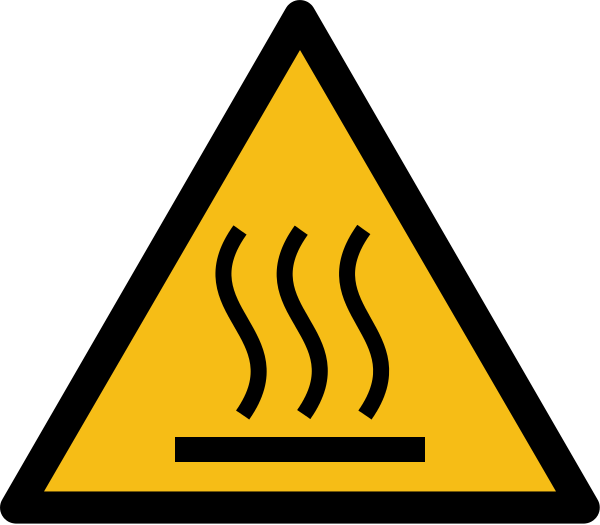
\includegraphics[width=2.5cm]{hot-surface.png} & 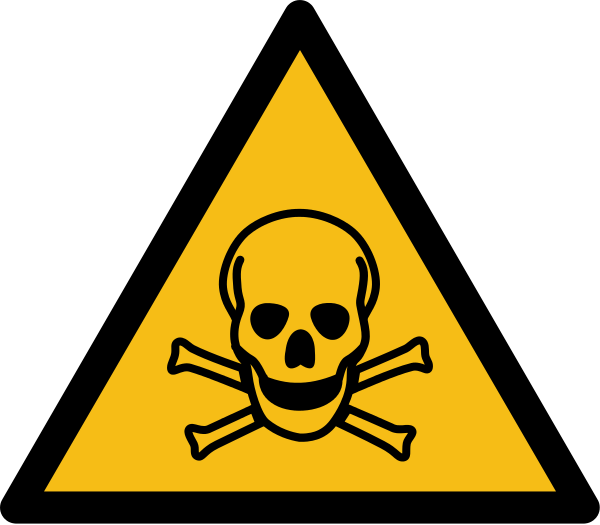
\includegraphics[width=2.5cm]{toxic.png}\\
		\textbf{Achtung heiße Oberfläche!} & \textbf{Achtung Giftig!}
	\end{tabular}
\end{center}
Die Lötspitzen sowie der Luftstrom der Heißluft erreichen Temperaturen von 400°C! Verbrennungsgefahr! \\\\
Wir verwenden bleihaltiges Lötzinn! Dies ist beim Einatmen und Verschlucken gesundheitsschädlich. Das Lötzinn enthält Kolophonium welches allergische Reaktionen hervorrufen kann.
Es muss immer die Lötrauchabsaugung verwendet und die Hände nach den Arbeiten gewaschen werden.
\section{Technische Daten}
 \begin{tabular}{|l|l|}
 	\hline
 	Hersteller & XYTRONIC\\
 	\hline
	Leistung & 900W \\
	\hline 
	Löttemperatur & 150 - 480°C\\
	\hline
	Entlöttemperatur & 300 - 450°C\\
	\hline
	Heißlufttemperatur & 100 - 480°C\\
	\hline
\end{tabular}
\newpage
\section{Bedienung}
\subsection{Allgemeines}
Benötigte Funktionen mit $\triangledown$-Taste aktivieren.\\
Nicht (mehr) benötigte Funktionen mit $\triangle$ +SET deaktivieren.\\
Nach der Arbeit Schalter der Steckdosenleiste ausschalten.
\subsection{ESD-sicheres Arbeiten}
\begin{itemize}
	\item Lötspitze und Entlötspitze der Lötstation sind geerdet (Mit Schutzleiter der Steckdose
	verbunden).
	\item Die graue Matte ist über einen 10 M$\Omega$ Schutzwiderstand ebenfalls mit dem Schutzleiter der
	Steckdose verbunden.
	\item Um dich selbst zu erden, verwende ein Erdungsarmband und befestige dies am vorderen
	Druckknopf der Matte oder an einem freien Druckknopf des gelben Erdungssteckers an der
	Steckdosenleiste.
\end{itemize}
\subsection{Löten (linkes Bedienelement)}
\begin{itemize}
	\item empfohlene Temperatur für Through-Hole: ca. 300°C
	\item empfohlene Temperatur für SMD: ca. 260°C
	\item Lötkolben vor der Arbeit immer erst auf Betriebstemperatur aufheizen lassen.
	\item Spitze zur besseren Wärmeleitfähigkeit vor dem Ansetzen verzinnen. Gegebenenfalls Lötfett
	benutzen.
   \item Spitze stets sauber halten, Metallwolle in der Halterung zum Abstreifen verwenden.
\end{itemize}
\subsection{Entlöten (mittleres Bedienelement)}
\begin{itemize}
	\item Solltemperatur: ca. 370°C
	\item \textbf{Pumpe nicht betätigen, bevor Temperatur erreicht ist!} Das Lötzinn härtet sonst durch die
	rasche Erkaltung bereits im Absaugkanal aus und verstopft die Düse.
	\item Der Aufheizprozess dauert mehrere Minuten. Für einzelne, wenige Lötstellen ist es
	empfehlenswert, auf den mechanischen Sauger zurückzugreifen. Geht schneller.
\end{itemize}
\subsection{Heißluft (rechtes Bedienelement)}
\begin{itemize}
	\item Erst AIR ganz aufdrehen, dann Heizung auf ON stellen.
	\item \textbf{Nach Gebrauch der Heißluft erst Heizung ausschalten} ($\triangle$+SET) und warten, bis die Luft
	aus der Düse kalt ist. \textbf{Dann erst AIR wieder runter drehen.}
\end{itemize}
\end{document}
